\documentclass[12pt,onecolumn]{article}

% Page dimensions
\setlength{\hoffset}{-1in}
\setlength{\voffset}{-1in}
%\setlength{\headsep}{-0.2in}

\setlength{\oddsidemargin}{1.0in}
\setlength{\evensidemargin}{1.0in}
\setlength{\textwidth}{6.5in}
\setlength{\textheight}{9in}

%\setlength{\columnsep}{0.3in}

% Packages
\usepackage{fancyhdr}
\usepackage{lastpage}
\usepackage{abstract}
\usepackage{amsmath, amssymb} 
\usepackage{epsfig}
\usepackage{subcaption} 
\usepackage[english]{alg}
\usepackage[usenames,dvipsnames]{color}
\usepackage{empheq}
%\usepackage[hidelinks]{hyperref}
\usepackage{hyperref}
\usepackage{sectsty}

\usepackage{morefloats}

% Packages for notes, testing, etc.
\usepackage{todonotes}
\usepackage[inline]{showlabels}

\showlabels[\color{blue}]{cite}
\showlabels[\color{blue}]{ref}

%% ============================================================

% Macros
\newcommand{\CHRONO}{{\sffamily{{Chrono}}}}
\newcommand{\ChronoFEA}{{\sffamily{Chrono}}::FEA}
\newcommand{\ChronoVehicle}{{\sffamily{Chrono}}::Vehicle}
\newcommand{\ChronoFSI}{{\sffamily{Chrono}}::FSI}
\newcommand{\ChronoGranular}{{\sffamily{Chrono}}::Granular}
\newcommand{\ChronoParallel}{{\sffamily{Chrono}}::Parallel}
\newcommand{\ChronoDistributed}{{\sffamily{Chrono}}::Distributed}
\newcommand{\ChronoOpenGL}{{\sffamily{Chrono}}::OpenGL}

%% ============================================================

% Styles

\definecolor{my-gray}{gray}{0.4}

% First page header
\fancypagestyle{firststyle} {
	\lhead{}
	\rhead{
	\footnotesize
	\textbf{2017 NDIA GROUND VEHICLE SYSTEMS ENGINEERING AND TECHNOLOGY SYMPOSIUM}\\
	\textbf{\sc Modeling \& Simulation, Testing and Validation (MSTV) Technical Session}\\
	\textbf{\sc August 8-10, 2017 -- Novi, Michigan}	
	}
	\chead{}
	%
	\lfoot{}
	\cfoot{}
	\rfoot{}
}

% All other pages (header and footer)
\pagestyle{fancy}
\fancyhf{}
\rhead{
	\color{my-gray}
	\footnotesize Proceedings of the 2017 Ground Vehicle Systems Engineering and Technology Symposium (GVSETS)
	}
\cfoot{
	\color{my-gray}
	\footnotesize
	{\FooterTitle}\\
	Page \thepage~of~\pageref{LastPage}
}

\renewcommand{\headrulewidth}{0pt}

% Font and styles for sections
\allsectionsfont{\fontsize{12}{15}\selectfont}

\renewcommand{\abstractname}{ABSTRACT}
\renewcommand{\refname}{REFERENCES}

%% ============================================================

\title{\bf\large PERFORMANCE ANALYSIS OF CONSTANT SPEED LOCAL OBSTACLE AVOIDANCE CONTROLLER USING AN MPC ALGORITHM ON GRANULAR TERRAIN}

\newcommand{\FooterTitle}{Performance analysis of obstacle avoidance algorithm on granular terrain}

\author{
	{\bf Nicholas Haraus}\\
	Dept. of Mechanical Engineering\\
	Marquette University\\
	Milwaukee, WI
}

\newcommand{\MyAbstract}{
	A Model Predictive Control (MPC) LIDAR-based constant speed local obstacle avoidance algorithm has been implemented on rigid terrain and granular terrain in {\CHRONO} to examine the robustness of this control method. 
	Provided LIDAR data as well as a target location, a vehicle can route itself around obstacles as it encounters them and arrive at an end goal via an optimal route.
	Using {\CHRONO}, a multibody physics API, this controller has been tested on a complex multibody physics HMMWV model representing the plant in this study. A penalty-based DEM approach is used to model contacts on both rigid ground and granular terrain. We draw conclusions regarding the MPC algorithm performance based on its ability to navigate the {\CHRONO} HMMWV on rigid and granular terrain.  A novel simulation framework has been developed to efficiently simulate granular terrain for this application.
}

%% ============================================================
\pagenumbering{roman}
\begin{document}
\onecolumn
\begin{titlepage}
	\date{}
	\maketitle             % full width title
	\thispagestyle{firststyle}
	\MyAbstract
	\\\vspace{0.2in}
\end{titlepage}


%% ============================================================
\section{ACKNOWLEDGEMENTS}\label{s:Acknowledgements}

%% ============================================================
\newpage
\section{TABLE OF CONTENTS}\label{s:TableofContents}
\tableofcontents

%% ============================================================
\newpage
\section{LIST OF TABLES}\label{s:tables}
\listoftables

%% ============================================================
\newpage
\section{LIST OF FIGURES}\label{s:figures}
\listoffigures

%% ============================================================
\newpage
\section{LIST OF EQUATIONS}\label{s:equations}
%\listofequations

%% ============================================================
\newpage
\pagenumbering{arabic}
\setcounter{page}{1}
\section{INTRODUCTION}\label{s:introduction}

Obstacle avoidance is a crucial capability for Autonomous Ground Vehicles (AGVs) of the future. This refers to a ground vehicle's ability to sense its surrounding environment, develop an optimal path around the obstacles in the environment, generate optimal control commands to satisfy that path, and physically navigate around the obstacles safely and to a desired endpoint. Safety is defined as avoiding collisions as well as enforcing limitations on excessive sideslip or tire lift-off. An ideal control algorithm is one that is capable of pushing a vehicle to its performance limits by using knowledge of its dynamic capabilities and surrounding environmental conditions, while still enforcing strict safety requirements. Although previous work has demonstrated use of Model Predictive Control (MPC) algorithms for obstacle avoidance on wheeled vehicles, more work is required to test the fidelity of these algorithms and determine where improvements are needed. One area in which MPC algorithms have yet to be tested is their ability to control a wheeled vehicle on granular terrain. Up to this point, the terrain has been assumed to be rigid and flat. Performance of MPC algorithms on deformable terrain raise additional questions. Do the current most commonly used vehicle models perform successfully within an MPC algorithm on deformable terrain? The present work evaluates, through numerical simulation, the robustness and validity of an MPC algorithm with different vehicle models in an environment more similar to what an off-road military vehicle would experience in combat. This controller could be applied to any car-like wheeled vehicle.

The remainder of this paper is organized as follows.  In Section~\ref{s:background} we provide overviews of the MPC-based local obstacle avoidance algorithm and the {\CHRONO} multiphysics package used as the test environment. In Section~\ref{s:methodology} we describe the {\ChronoVehicle} HMMWV vehicle model used in this study as the plant model to be controlled and our proposed method for simulating a vehicle driving on deformable terrain over large distances. Then, the specific MPC LIDAR-based local obstacle avoidance controller used for this study is presented. We introduce the different simplified, lower-fidelity analytical vehicle models used in the MPC algorithm to predict the {\CHRONO} vehicle behavior. We also provide descriptions of the test cases considered for this study and a summary of the metrics used to compare performance of the various tested combinations. In Section~\ref{s:results} we present the results of the tests outlined in the previous section and provide comparisons when the internal controller vehicle model is varied and when the terrain is changed from rigid to granular. Section~\ref{s:conclusion} wraps up the paper and presents potential future work based on the results of this study.
\todo[inline]{fix this paper organization section}

%% ------------------------------------------------------------

\subsection{Problem Summary}\label{ss:ProblemSummary}

Regarding the MPC control algorithm, many studies have been performed previously to validate its potential to develop local obstacle avoidance controllers. Specifically, studies by Liu, Jayakumar, Overholt, Stein, and Ersal explored the implementation of an MPC local obstacle avoidance algorithm in AGV’s. The research group tested a steering controller for an AGV on rigid flat terrain \cite{ModelFidelity2013}, then a combined steering and speed controller \cite{SpeedSteer2015}, and finally studied the role of model fidelity in the implementation of the MPC algorithm \cite{ModelFidelity2016} to understand how detailed the controller model needs to be to effectively and quickly control the vehicle. However, in these studies and those performed before them, the AGV has been tested on rigid flat terrain, an assumption which does not hold when driving a vehicle in reality. Therefore, the research for this thesis will perform  studies on the promising models from \cite{ModelFidelity2016} and test them on granular terrain to understand how changing the ground from rigid and flat to granular affects the controlled AGV performance.

This research also addresses another larger problem for the military. The North Atlantic Treaty Organization (NATO) is seeking to replace their current NATO Reference Mobility Model (NRMM) \cite{NATONRMM}. The current NRMM is an empirically based computer model developed during the 1970s, which computes tactical mobility metrics by correlating engineering level performance of various ground vehicle systems with different terrain conditions, allowing for successful comparison of these ground systems and capabilities over varied terrain surfaces, obstacles, vegetation, weather scenarios, grades, and other features which can adversely impact ground vehicle performance. NATO seeks to replace this older model with a new physics-based computer simulation solution which can still answer the same questions as the older model, but can then be extended past situations with only empirical results. One of the key areas of work in this group effort is the ability to develop and deliver to the vehicle go-nogo maps of upcoming terrain, either from recent satellite imagery or other sorts of sensors. With this research, the development of this simulation and test will seek to control an AGV only with the sensor data or terrain inputs provided by the mission planner. Any research achieved relating to vehicle mobility across a variety of terrains can help with the NRMM effort. 

Significant studies have been carried out and work accomplished testing the MPC Algorithm and validating Chrono as a viable program for Multibody simulations. However, the two topics have not combined to be tested together. The MPC algorithm has been tested on rigid flat terrain, yet with Chrono Parallel one has the ability to simulate granular terrain if desired with reasonable runtimes. Therefore, one can develop a simulation of a vehicle on granular terrain with scattered obstacles in Chrono Parallel, and then use the MPC algorithm from \cite{ModelFidelity2016} to control that simulated vehicle. Doing so would benefit both the simulations field and the controls field. By bridging the gap between these two areas, those designing the control algorithms have a quicker and less expensive method of testing a control algorithm on a full vehicle on a variety of landscapes to gain quick understanding of how well their controller behaves. On the other hand, developing this sort of simulation improves the amount of applications Chrono Parallel can be used in. This research has performd higher fidelity testing of the control algorithm than has previously been accomplished, a step which is necessary if this algorithm is to eventually be implemented in an actual vehicle. 

	The uniqueness of this research comes from two areas: controls and simulation. Most Chrono simulations created so far do not test any sort of complex control algorithm for an autonomous vehicle. More interest is placed in understanding vehicle mobility over different terrains. However, this research does test an autonomous vehicle and its ability to navigate around local sensed obstacles. Therefore, a frmework has been developed to allow the simulated vehicle to “sense” obstacles in the area and generate its own commands while it navigates across the terrain instead of relying on externally supplied commands. Can this MPC control algorithm generate the appropriate commands to navigate a vehicle through an obstacle field? On the controls side, this is a unique effort as well. As mentioned, the MPC algorithm has yet to be tested on granular terrain. However, considering an AGV will be driving off road on soil or sand, this is an appropriate next step for testing. This research answers the question of if simulation can be used to effectively test an autonomous vehicle on granular terrain. Computationally this requires a lot of resources, but if a team can test their control algorithm on the computer before going out to the test field with a vehicle, this could save both time and money for that team.

\todo[inline]{copied from thesis outline, needs to be updated}

%% ------------------------------------------------------------

\subsection{Literature Review}\label{ss:LiteratureReview}

Many obstacle avoidance algorithms have been developed in the past that allow for smooth, continuous, fast motion of an AGV through an obstacle field. Early algorithms were primarily developed and tested on small ground robots and mainly focused on finding a collision free path. However, they did not necessarily guarantee optimality or the vehicle's ability to achieve that prescribed collision-free path. Some early researched algorithms were developed using artificial potential methods. Applied to a manipulator moving through space, the philosophy of the potential field approach can be summarized as: "The manipulator moves in a field of forces. The position or target to be reached is an attractive pole while all obstacles are repulsive surfaces for the manipulator parts"~\cite{Khatib1986}. Khatib described the formulation and implementation of the artificial potential field concept towards obstacle avoidance. Using the kinematic relationships of the system to be controlled, a Lagrangian formulation is used to develop the equations of motion of the system. An artificial potential field is created that is nonnegative continuous and differentiable whose value goes to infinity as the vehicle approaches an obstacle. The overall artificial potential function is then a sum of the contributing potential fields caused by each of the obstacles within the obstacle field. Each of the obstacles are modeled as a composition of primitives with analytical equations representing their collision envelopes. Khatib successfully implemented this obstacle avoidance algorithm real-time in \textit{Control in Operational Space of a Manipulator-with-Obstacles-System} (COSMOS)with links and moving obstacles \cite{Khatib1986}. 

Rimon and Koditschek then presented a technique for constructing artificial potential fields that could bring a bounded-torque actuated robot to a desired configuration without hitting obstacles ~\cite{Rimon&Koditschek1992}. Their formulation works for any n-DOF robot whose configuration space happens to be a generalized sphere world. However as with \cite{Khatib1986}, this formulation requires \textit{a priori} knowledge of the topology of the obstacle field. Therefore the implementation of the algorithm at the point of publication of \cite{Rimon&Koditschek1992} is infeasible for unknown obstacle fields. 

Vector Field Histogram methods were then researched due to their ability to to navigate a robot through an unknown environment where topology is not known \textit{a priori}. The Vector Field Histogram (VHF) method allows the detection of unknown obstacles and avoids collisions as it steers a mobile robot to some end destination \cite{Borenstein&Koren1991}. The VHF method models the world as a two-dimensional Cartesian histogram grid and continuously updates the grid based on the input on-board sensor data. The algorithm reduces the histogram to a one-dimensional polar histogram around the current robot location such that each sector of the polar histogram has a polar obstacle density associated with it. The algorithm then selects the sector with a low obstacle density and aligns the robot's steering with that sector \cite{Borenstein&Koren1991}. The VHF method outlined in \cite{Borenstein&Koren1991} successfully navigated a mobile robot though an obstacle field at an average speed of 0.6-0.7 m/s. This method is a local path planner, so there is no way of it purposefully following a globally optimal path. This algorithm is also susceptible to dead end situations and local minima \cite{Borenstein&Koren1991}.

In a much more recent study, Gong and Duan proposed a multi-strategy navigation method to combat some common problems with autonomous vehicle navigation \cite{Gong&Duan2009}. The two common problems addressed were the vehicle reaching a local minimum and the vehicle navigating into a dead end. Both scenarios result in the vehicle remaining stuck forever with many algorithms. The proposed multistrategy algorithm identifies the current state of the vehicle and determines which navigation strategy is best for the current moment. Vector Polar Histogram is used until the vehicle gets stuck at a dead end or local minimum. The controller then switches modes to a wall-following algorithm, forcing the vehicle to find a wall and follow it until out of the dead end. If the vehicle is stuck in a local minimum, the the controller may switch to a move-towards-goal algorithm forcing the vehicle to progress straight to the goal if not blocked by obstacles for a short time until away from the local minimum. This would also apply to the situation where a vehicle's path to the goal is clear, but the goal is right next to a obstacle and therefore the Vector Polar Histogram prevents that path from being considered as a possibility. This method successfully navigated a vehicle in both simulation and real life at a top speed of 1 m/s \cite{Gong&Duan2009}.

Dynamic Window Approaches at their roots are most similar to the MPC algorithm used for the research of this thesis. Fox, Burgard, and Thrun focus specifically on the reactive avoidance of collisions with obstacles by a robot \cite{Fox1997}. A dynamic window approach is proposed that deals with constraints imposed by velocity and acceleration limits. Steering commands are computed periodically thus avoiding the complexity of a general motion planning problem. First, they consider velocities that result in circular trajectories. Then, only velocities that can be reached within the next time window are considered, largeley decreasing the search space forming the dynamic window. Admissible velocities are weighed by an objective function. In experiments, this method successfully navigated a B21 mobile robot at a top speed of 0.95 m/s \cite{Fox1997}.

Brock and Khatib then proposed a global dynamic window approach to obstacle avoidance that combines path-planning and real-time obstacle avoidance algorithms to generate robot motions to complete a task and still remain safe in an unknown environment \cite{Brock&Khatib1999}. As the robot moves through the environment, it builds an occupancy grid based off sensor input data to represent the connectivity of free space. This allows the robot to learn about its environment without any global \textit{a priori} knowledge of the obstacles. The global dynamic window approach combines the reactive collision avoidance of the dynamic window approach of \cite{Fox1997} with a global, local minima-free navigation function \textit{NF1}. An objective function is developed to choose the best path forward. This global dynami window approach was successfully tested with a synchro-driven mobile robot Noman XR4000 at 1.0 m/s \cite{Brock&Khatib1999}.

Kunchev, Jain, Ivancevic, and Finn presented a review and comparison of path planning and obstacle avoidance techniques including those previously mentioned. Each obstacle avoidance method has its own benefits and disadvantages. It seems at this point the issue of local minima is significant for all developed algorithms. All the mentioned techniques need more development to be applied to a car-like vehicle at higher speeds \cite{Kunchev1999}. More recent research aims to take these early collision avoidance algorithms and adapt them towards the navigation of high speed AGV's. The motion of these AGV's is not as simple as the small robots the algorithms were intially developed for in that the AGV cannot instantaneously move in any direction. Ignoring the effects of slip, a car-like AGV will move in its heading direction. Newer research has aimed to build upon or even combine previously mentioned algorithms for the application towards car-like AGV's.

Shimoda, Kuroda, and Iagnemma proposed a potential field based method of navigating an unmanned ground vehicle at high speeds across sloped and rough terrains \cite{Shimoda&Kuroda&Iagnemma2007}. With this proposed method, a potential field is generated in a two dimensional trajectory space of the path curvature and longitudinal velocity. The potential field in generated based on dynamic constraints, terrain slopes, obstacle proximities, and the target location. A maneuver is selected within a set of performance bounds based on the local potential field gradient. Each maneuver is mapped to the low level commands necessary to execute that maneuver. This method has successfully been tested at a speed of 7 m/s \cite{Shimoda&Kuroda&Iagnemma2007}.

Koren and Borensteain the performed a study presenting a systematic overview of the downfalls of potential field methods \cite{Koren&Borenstein1991}. Four main drawbacks are noted and described. First, a well-documented issue is trap situations due to local minima. Second, even though the controlled robot may be slightly smaller than a certain gap between two obstacles, the combined repulsive force from the two obstacles prevents the robot from passing through gaps it should be able to. Third, the robot motion exhibits oscillatory behavior near obstacles. This same behavior is seen in the fourth noted downfall where if a robot is moving through a narrow-walled passage, the robot will oscillate close to each wall throughout the whole passafe again due to the nature of the developed potential field and repulsive forces. For certain applications, potential field methods may be appropriate due to simple, elegant, and quick navigation of the robot through the obstacle field. However, Rauth stability criterion presented in \cite{Koren&Borenstein1991} prove this method would not be stable as vehicle mass and speed increase. This therefore makes the artificial potential field method unsuitable for the research of this study.. These drawbacks have been experimentally proven and motivated a move by Koren and Borenstein away from potential field methods \cite{Koren&Borenstein1991}.

To address the issue of optimality, more rigorous approaches have been developed leveraging the Model Predictive Cotnrol approach. With this method, control action is obtained by solving a finite horizon open-loop optimal control problem over a receding horizon.

Findheisen and Allg{\"o}wer provide an introduction to nonlinear Model Predictive Control \cite{Allgower&Findeisen2002}. Nonlinear MPC methods are being explored due to the method's ability to incorporate design driven constraints into the robot control. As time goes on, our systems are becoming subject to more safety and environmental constraints making the application of previously mentioned methods difficult. With nonlinear MPC, it is not too difficult to add more system constraints to the optimal control problem solved each time step. Multiple applications and derived nonlinear MPC methods are presented as well in \cite{Allgower&Findeisen2002}. MPC is therefore a promising approach for obstacle avoidance due to its capability to handle input saturation, system nonlinearities, and design state constraints in a dynamic environment.

Ogren and Leonard present the Dynamic Window Approach for fast and safe obstacle avoidance in unknown environments and recast the approach in a continuous nonlinear framework, drawing many similarities to MPC \cite{Ogren&Leonard2005}. A method for generating a navigation function with a single unique minimum is presented. In this study, the control input space is discretized for a computationally tractable version of MPC, and exhaustive search is used to identify the best control input choice. Of all the control input possibilities, there always exists one such that the robot will be able to stop before hitting any obstacle to insure safety \cite{Ogren&Leonard2005}.

Primbs, Nevisti, and Doyle explore Control Lyapunov Functions (CLF) and Receding HOrizon Control or MPC approaches to nonlinear control \cite{Primbs&Nevistic1999}. Comparisons are made between the two methods and it is noted that they seek to solve the same problem optimally and some properties of each method are complementary to one another. The CLF methods are best interpretted in the context of Hamilton-Jacobi-Bellman equations while MPC relates more closely to a Euler-Lagrange framework. The CLF provides a global optimal solution, but the partial differential equation one must solve is very difficult and computationally infeasible. The MPC approach instead allows for on-line computation of an optimal solution locally, and resolves this problem every time step specified. The problem is only solved over a fixed time horizon. However, it is difficult to apply Lyapunov Stability Theory to this MPC method where numerical techniques are used to solve for optimal solutions. Also, the relation between time horizon length and stability are not necessarily linear as noted by results from experiments \cite{Primbs&Nevistic1999}. 

Tahirovic and Magnani propose a passivity based MPC control for Robot Navigation through rough terrain \cite{Tahirovic&Magnani2010}. This method boasts simplicity of application for all vehicles as long as one can accurately model them. A virtual model of the vehicle is then made using shaped energy. The algorithm quantifies roughness of the terrain and uses this parameter when analyzing the cost of a specified path. The roughness is expressed as the relative height of the terrain locally. Simulations have proven successful navigation of a vehicle through hilly terrain, yet there is no mention of how the terrain data would actually be obtained \cite{Tahirovic&Magnani2010}. This passivity based MPC method can be applied on-line, but this would only be feasible if there was some sort of sensor and data analysis algorithm which can sense the local terrain roughness.

Bevan, Gollee, and O'Reilly proposed a new method for trajectory generation for road vehicle obstacle avoidance using convex optimization \cite{Bevan&Gollee2010}. The dynamics of a vehicle is a very nonlinear case which on the surface poses a non-convex optimization problem when searching for an optimal path trajectory. This study used their method on a vehicle performing an aggressive double lane change maneuver with the intent of designing a quick emergency obstacle avoidance algorithm for when cars either need to stop immediately or turn to move around an incoming obstacle. Most avoidance systems solely slow the vehicle down to prevent collision with a hazard in the vehicle heading direction. The optimization is performed in three stages in which each stage includes different assumptions to frame the problem as a convex optimization problem. The first stage solves for a trajectory assuming no slip, the second assumes slip but constant speed, and the third uses the values from the previous stages to insert to non-convex expressions and holds those terms constant. This study successfully simulated a general wheeled vehicle performing an optimal double lane change maneuver \cite{Bevan&Gollee2010}.

Nanao and Ohtsuka presented a nonlinear MPC algorithm which finds a solutions using continuation/generalized minimal residual (C/GMRES) algorithm to find a solution \cite{Nanao&Ohtsuka2010}. The algorithm was tested successfully in simulation and though runtimes are not yet quick enough for real-time implementation, they expect it in the near future of this paper. Tire ground interactions are modeled using the Pacejka Magic Formula. A friction circle is used to quickly determine the maximum friction force able to be generated and this is used to create an "unavoidable region" in which the vehicle is unable to avoid hitting the obstacle \cite{Nanao&Ohtsuka2010}. However, this method relies heavily on accurate modeling of the ground tire interactions.

Gao, Lin, Borrelli, Tseng, and Hrovat presented and tested two different MPC algorithms for obstacle avoidance \cite{Gao&Borrelli2010}. The first algorithm is a one level MPC algorithm. The algorithm combines the requirements of obstacle avoidance and the optimal trajectory planning into one step, solving a highly nonlinear optimal control problem within the horizon each time step. The objective function includes a proximity term which increases as the vehicle approaches an obstacles. The second algorithm is a two-level approach. A high-level path planner calculates an optimal trajectory for the vehicle disregarding any obstacle information. A low level algorithm then calculates the optimal control inputs that both route the vehicle around obstacles and maintain the vehicle along the desired trajectory. While both algorithms were implemented in realtime successfully on an icy road performing a double lane change maneuver, the two-level approach was successful at speeds of 55 kph while the one level could only be implemented up to 40 kph. Computational runtimes were compared and show the two-level approach runs much quicker than the one-level approach and shows promise for hierarchical MPC methods in the future \cite{Gao&Borrelli2010}.

The two-level MPC method was developed further and addressed the issue of the vehicle model predicting infeasible trajectories for the vehicle in the high-level planner \cite{Gray&Gao2012}. Instead, motion primitives are used to develop a high-level trajectory assembled from trims which are connected by maneuvers. Possible trims are straight, left turn, right turn, drift left, and drift right. Maneuvers connect two trims. The possible maneuvers include straight to left turn, left turn to straight, stright to drift right, etc. This method proved successful in simulation. In experiments, a vehicle was able to successfully avoid obstacles, but no mention is made of the vehicle speed \cite{Gray&Gao2012}.

Abbas, Eklund, and Milman analyzed the possible realtime implementation of a nonlinear MPC algorithm for obstacle avoidance using Simulink and simulating the vehicle as a full Carsim nonlinear multibody vehicle \cite{Abbas&Eklund2012}. Offline a trajectory is generated guiding the vehicle from a start point to the desired end location. Then on-line each controller time step a cost function is used to weigh possible trajectories and deviations from the reference trajectory are penalized. A pointwise potential function is used to increase cost as the vehicle gets closer to any obstacle. Simulation results showed the vehicle is capable of navigating around a single obstacle. The cost function is minimized using the gradient descent optimization method. The amount of time to find an optimal path in the simulation varies depending on the scenario the vehicle is in at each time step. A vehicle in close proximity to an obstacle will take longer to pick the best path than a vehicle in free space pointed towards the goal. Warm starting is used during the optimization routine to help quicken the optimization process, but there are still many time step scenarios where the amount of time needed to calculate a best path exceeds the available time the controller has to find that path \cite{Abbas&Eklund2012}.

A nonlinear MPC algorithm was then proposed for realtime obstacle avoidance that uses the software ACADO to autogenerate C-code to perform the high-level trajectory planning \cite{Frasch&Gray2013}. This increases algorithms speeds to the point where even with a complicated vehicle model, nonlinear tire model, and wheel dynamics considered, this proposed method was able to perform computations quickly enough to control a vehicle realtime at 10 m/s on rigid flat ground \cite{Frasch&Gray2013}.

Researchers have proposed a fast motion planner that uses a half-car dynamical model for a wheeled vehicle \cite{Jeon&Cowlagi2013}. A fast local steering algorithm is developed to increase runtimes and splits into a geometric path planning step and then an optimal time parameterization step. The three control inputs are steering angle and the longitudinal slips of the fron and rear tires much like a rally car driver would control. Simulation results support the realtime implementations of this obstacle avoidance controller \cite{Jeon&Cowlagi2013}.

Several studies have been performed examing MPC-based techniques for car-like vehicle collision avoidance. A MPC algorithm was developed that controls the braking and steering to better control the vehicle during a double lane change maneuver \cite{Falcone2007}. This algorithm was tests on a snowy road. In experiments, a controller that controlled both braking and steering performed better than an algorithm controlling steering alone \cite{Falcone2007}.

Gray, Ali, Gao, Borrelli, and Hedrick used a MPC algorithm to maintain driver safety by keeping a vehicle within its lane \cite{Ali&Gray2013}. The control has an internal four wheel vehicle model as well as a driver model, allowing the controller to predict driver commands and intentions. The controller aims to minimize its own input so that only when the driver is in danger such as departing from the lane will the controller take action. Otherwise, it seeks to maintain safety constraints so that the controller only intervenes when it senses safety constraints may be violated. Simulation results proved successful, but when implemented in real life at a Volvo facility, the only issue encountered was minor breaking of a safety constraint. This however was due to sensor delay and in the future this delay will be accounted for in the algorithm \cite{Ali&Gray2013}.

Beal and Gerdes proposed a solution to the issue of vehicle stabilization control near the limits of handling \cite{Beal&Gerdes2013}. Normally, an ESC works by using a linear model of a vehicle to predict driver intent and when the vehicle deviates past a threshold of the allowed deviation between driver intent and vehicle behavior, then the controller activates and stabilizes the vehicle. However, this method does not work when the vehicle is being operated near the stable vehicle limits such as by an experienced driver because the linearized vehicle model is linearized about a conservative point for production level cars. The vehicle behavior near its dynamic limits is nonlinear and does not match the linearized model. Therefore, an MPC based controller was proposed and tested that operates at two levels and quickly enough for realtime implementation. The controller has two objectives. The first is to keep the vehicle inside of the safe-handling envelope and respond appropriately in case the vehicle leaves this safe envelope. The second objective is to allow the controller to track the driver's intended trajectory. Overall the controller was able to successfully achieve these objectives through experiments with Stanford's PI vehicle testbed \cite{Beal&Gerdes2013}.

\todo[inline]{finish lit review}






%% ------------------------------------------------------------

\subsection{Objectives and Methodology}\label{ss:ObjectivesMethodology}

The goal of this research is to understand how model fidelity of the controller model affects overall performance of the obstacle avoidance controller. This leads to a better understanding of vehicle dynamics and performance on granular terrain as well as promotes the development of a controller designed for general terrain travel in the future. Simulating a vehicle on granular terrain in such scenarios introduces additional challenges related to the sheer number of necessary particles required to properly model the desired terrain patch. This challenge has been addressed by employing a simulation framework for granular terrain described later in this paper.

The present study has the following three objectives:
\begin{enumerate}
\item
Study the performance of the MPC Controller on granular terrain as compared to that on rigid terrain.
\item
Analyze the impact of fidelity of the internal controller model on speed and performance of the obstacle avoidance controller.
\item
Showcase the potential of controller testing in a high fidelity virtual test environment with {\CHRONO} to assist with initial control algorithm development before physical implementation for vehicular applications.
\end{enumerate}

From previous literature research, this MPC algorithm has been tested successfully on flat rigid terrain. However, using Chrono Parallel one has the capabilities to develop a simulation of a vehicle on hilly, deformable, and even granular terrain. In this research, Chrono Parallel is used to develop a simulation of a AGV driving on customizable granular terrain through a user defined obstacle field to a defined target location. Chrono already possesses the ability to create new geometries easily with a modular framework, so one will then be able to easily create their own obstacle field for the vehicle to maneuver through. Using theory and developments from \cite{ModelFidelity2016}, the MPC algorithm has been implemented in the simulation to determine optimal steering commands for the AGV. Tests similar to those executed in \cite{ModelFidelity2016} were conducted within this simulation on rigid flat terrain for the two models presented previously to confirm the controller operates appropriately. The algorithm was then tested on granular terrain to understand how controlled vehicle performance changes on granular terrain versus previously tested rigid ground simulations. The MPC algorithm solves a very large optimization problem to determine the quickest safe path to the destination. An exhaustive search based method was used to solve this optimal control problem. Improvements were explored to boost vehicle performance on granular terrain and are discussed at the end of this paper.

/todo[inline]{copied from thesis outline, adjust}

%% ============================================================

\section{THEORETICAL BACKGROUND}\label{s:background}

\subsection{{\CHRONO} Multibody Physics Package}\label{ss:Chrono}

The physics modeling and simulation capabilities are provided by the multiphysics open-source package {\CHRONO}~\cite{Chrono2016}. The core functionality of {\CHRONO} provides support for the modeling, simulation, and visualization of rigid multibody systems, with additional capabilities offered through optional modules. These modules provide support for additional classes of problems (e.g., finite element analysis and fluid-solid interaction), for modeling and simulation of specialized systems (such as ground vehicles and granular dynamics problems), or provide specialized parallel computing algorithms (multi-core, GPU, and distributed) for large-scale simulations.

%% ------------------------------------------------------------

\subsubsection{Vehicle Modeling}\label{sss:Chrono_Vehicle}
	
Built as a {\CHRONO} extension module, {\ChronoVehicle}~\cite{ChronoVehicle_paper} is a C++ middleware library focused on the modeling, simulation, and visualization of ground vehicles.
%
{\ChronoVehicle} provides a collection of templates for various topologies of both wheeled and tracked vehicle subsystems, as well as support for modeling of rigid, flexible, and granular terrain, support for closed-loop and interactive driver models, and run-time and off-line visualization of simulation results.

Modeling of vehicle systems is done in a modular fashion, with a vehicle defined as an assembly of instances of various subsystems (suspension, steering, driveline, etc.).  Flexibility in modeling is provided by adopting a template-based design. In {\ChronoVehicle}, templates are parameterized models that define a particular implementation of a vehicle subsystem. As such, a template defines the basic modeling elements (bodies, joints, force elements), imposes the subsystem topology, prescribes the design parameters, and implements the common functionality for a given type of subsystem (e.g., suspension) particularized to a specific template (e.g., double wishbone). Finally, an instantiation of such a template is obtained by specifying the template parameters (hardpoints, joint directions, inertial properties, contact material properties, etc.) for a concrete vehicle (e.g., the HMMWV front suspension).

For wheeled vehicle systems, templates are provided for the following subsystems:
{\em suspension} (double wishbone, reduced double wishbone using distance constraints, multi-link, solid-axle, McPhearson strut, semi-trailing arm);
{\em steering} (Pitman arm, rack-and-pinion);
{\em driveline} (2WD and 4WD shaft-based using specialized {\CHRONO} modeling elements, simplified kinematic driveline);
{\em wheel} (simply a carrier for additional mass and inertia appended to the suspension's spindle body);
{\em brake} (simple model using a constant torque modulated by the driver braking input).

In addition, {\ChronoVehicle} offers a variety of tire models and associated templates, ranging from rigid tires, to empirical and semi-empirical models (such as Pacejka and Fiala), to fully deformable tires modeled with finite elements (using either an Absolute Nodal Coordinate Formulation or a co-rotational formulation).  Driver inputs (steering, throttle, and braking) are provided from a {\em driver} subsystem with available options in {ChronoVehicle} including both open-loop (interactive or data-driven) and closed-loop (e.g., path-following based on PID controllers).

%% ------------------------------------------------------------

\subsection{MPC LIDAR-Based Local Obstacle Avoidance : History and Current Algorithm }\label{MPC}


\begin{figure*}
	\centering
	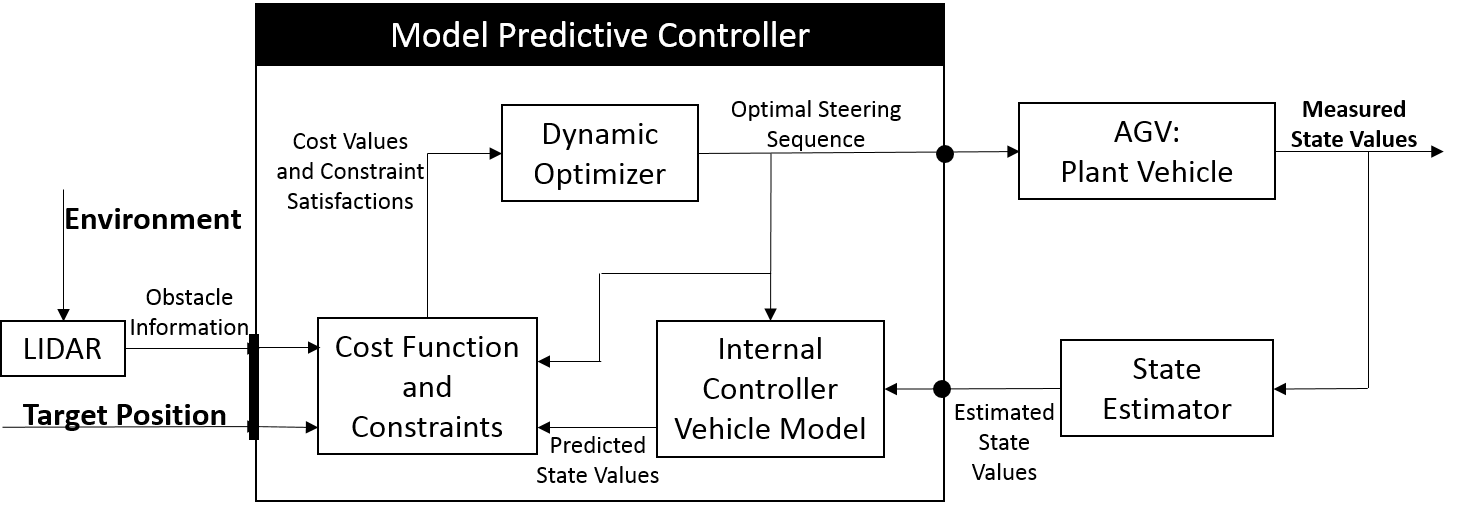
\includegraphics[width=0.75\textwidth]{Figs/MPCBlockDiagram.png}
	\caption{{\small Schematic of MPC LIDAR-Based Constant Speed Local Obstacle Avoidance Controller}}    
	\label{fig:MPC_schematic}
\end{figure*}

The concept of MPC is to use an internal model of the system one desires to control to predict and optimize future system behavior from the current system state and inputs ~\cite{Allgower&Findeisen2002}. The system behavior is predicted over some defined finite time horizon and the optimal control sequence over the prediction horizon is output. The control sequence is executed for an execution time smaller than the prediction horizon, and the whole process is repeated. The repetition of this process over time creates a feedback loop which continually controls the system, pushing it towards an optimal path.

For this study, the system to be controlled is an AGV. Consider an AGV located in a level environment without roads or any other structures to guide its motion and assume the AGV has a known global target position. Between the target position and the current vehicle position there may or may not be obstacles of unknown size. Using the MPC formulation outlined in~\cite{ModelFidelity2016}, the vehicle can navigate from the current position to the provided target position while avoiding obstacles as they are encountered. Obstacle information is assumed to be unknown a priori and only obtained through a planar LIDAR sensor. The MPC schematic is presented in Fig.~\ref{fig:MPC_schematic}.
%

\begin{figure}
	\centering
	\begin{subfigure}[b]{\columnwidth}
		\centering
		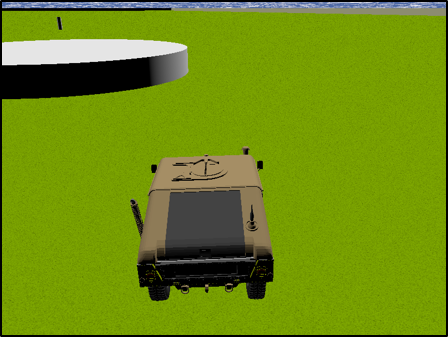
\includegraphics[width=0.8\columnwidth]{Figs/incomingObst.png}
		\caption{{\small 3D Visualization of LIDAR Encountering Obstacle}}   
		\label{fig:obstacle_field_3D}
	\end{subfigure}
	\hfill
	\begin{subfigure}[b]{\columnwidth}
		\centering
		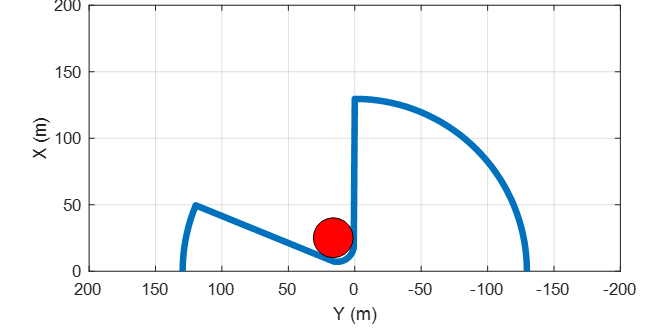
\includegraphics[width=\columnwidth]{Figs/obstLIDAR.png}
		\caption{\small LIDAR Sensed Safe Area}   
		\label{fig:obstacle_field_LIDAR}
	\end{subfigure}
	\caption{\small Sample obstacle field and LIDAR output}
	\label{fig:LIDARExample}
\end{figure}

The planar LIDAR sensor, mounted at the front center location of the vehicle, returns the closest obstacle boundary in all radial directions of the sensor at an angular resolution $\epsilon$. The sensor has a maximum range past which it cannot sense any obstacles. Therefore, if the closest obstacle boundary is greater than the LIDAR radius $R_{LIDAR}$, then the sensor returns $R_{LIDAR}$. The LIDAR sensor range is [$0^\circ$, $180^\circ$], with $90^\circ$ being the vehicle heading direction. Since the AGV considered here is driving along level ground, whether granular or rigid, a planar LIDAR sensor is sufficient. The sensor is assumed to have no delay and zero noise and can therefore instantaneously generate a safe area polygon assembled from the returned points from the LIDAR. An overhead view of the AGV encountering an obstacle and the generated LIDAR safe area polygon are presented in Fig.~\ref{fig:LIDARExample}. 
%
In this research, all of the obstacles are upright cylinders so a ray-circle intersection algorithm is used to determine when each LIDAR ray intersects with a nearby obstacle. 

\todo[inline]{insert description of the ray circle intersection algorithm used}

For the purpose of these simulations, the only outputs of the MPC algorithm are the steering signals. As shown in Fig.~\ref{fig:MPC_schematic}, the MPC algorithm is made up of the internal controller vehicle model, the cost function and constraints, and the dynamic optimizer. The internal controller vehicle model predicts the future states of the AGV for a given steering sequence. Herein, the internal controller vehicle model is varied from test to test between a 2-DOF vehicle model and a 14-DOF vehicle model, as detailed in further sections. Cost functions and constraints are used to formulate the optimal control problem using the equations from the vehicle model, and the resulting optimal control problem is solved using dynamic optimization.

Since the ability of finding and executing an optimal solution, rather than solution speed, is the primary focus here, an exhaustive search is used to find the optimal solution to the problem at hand. With this method, the steering sequence is discretized and a finite set of path possibilities are tested and weighed by a cost function. 

The MPC controller as formulated in~\cite{ModelFidelity2016} is used for this study. The cost function and constraints need to be specified to avoid collisions with obstacles and guarantee vehicle dynamical safety. The optimal control problem solved at each MPC time step consists of the following set of equations:

\begin{equation}\label{e:MPCCost}
J = s_T + wd 
\end{equation}
\begin{equation}\label{e:State_ODE}
\dot{\xi} = v\left[\xi\left(t\right),\zeta\left(t\right)\right] 
\end{equation}
\begin{equation}\label{e:InitialStates}
\xi\left(0\right) = \xi_0 
\end{equation}
\begin{equation}\label{e:SafeArea}
\tilde{S}\left[x\left(t\right),y\left(t\right)\right] \leq0  
\end{equation}
\begin{equation}\label{e:SteerLimit}
\left|\delta_f\left(t\right)\right| \leq\tilde{\delta}_{f,max}\left(U_0\right) 
\end{equation}
\begin{equation}\label{e:SteerRateLimit}
\left|\varsigma_f\left(t\right)\right| \leq\varsigma_{f,max} 
\end{equation}
\begin{equation}\label{e:TimeDomain}
t \in \left[0,T_P\right] \,.
\end{equation}

Equation~(\ref{e:MPCCost}) defines the cost function for this optimal control problem. This equation is a soft requirement which defines how the separate path possibilities are weighed against each other and how to determine which path is actually optimal. The cost function is comprised of two terms defined as:
%
\begin{equation}\label{e:DistanceCost}
s_T = \sqrt{\left[ x_G - x\left(T_P\right)\right]^2 + \left[y_G - y\left(T_P\right)\right]^2 }
\end{equation}
\begin{equation}\label{e:TurningCost}
d = \int \limits_0^{T_G} \left|\varsigma\left(t\right)\right| dt \,.
\end{equation}
%
Here, $s_{T}$ seeks to minimize the distance between the prediction end-location and the target position. A prediction path that guides the vehicle towards the closest location to the target will have the smaller $s_{T}$ term. The second term, $d$, aims to minimize the change in steering angle so that smoother, straighter paths are preferred over windy paths. A weighting factor $w$ is used to scale the influence of $d$ in the total cost.

Equations~(\ref{e:State_ODE}-\ref{e:TimeDomain}) are the constraints for this optimal control problem and represent hard requirements for vehicle safety and collision avoidance. Any paths that violate these constraints are not considered safe paths and are eliminated as potential options in this prediction window. Equation~(\ref{e:State_ODE}) defines a set of differential equations that describe the internal controller vehicle model, with the initial conditions of Eq.~(\ref{e:InitialStates}).

Equation~(\ref{e:SafeArea}) defines a safe area polygon, constructed from LIDAR data and including an additional safety buffer to account for vehicle size and to prevent collisions of the vehicle corners.  All points along paths found from Eqs.~(\ref{e:State_ODE})-(\ref{e:InitialStates}) must fall inside this safe area polygon.

Equation~(\ref{e:SteerLimit}) imposes a maximum limit on the steering angle, based on vehicle speed. This value is obtained from a lookup table which can be generated either experimentally or from simulation. Equation~(\ref{e:SteerRateLimit}) imposes a maximum limit on steering rate. Equation~(\ref{e:TimeDomain}) defines the time limits over which this optimal control problem is solved.

As noted above, Eq.~(\ref{e:State_ODE}) refers to an analytical vehicle model expressed as a set of differential equations which allow the controller to predict vehicle performance within the prediction horizon. The accuracy of the internal vehicle controller model should directly influence the driven vehicle's controlled performance. If the internal vehicle controller model poorly predicts a vehicle's response to inputs from the driver or the environment, then these deficiencies will be witnessed when attempting to control the driven vehicle and result in incorrect trajectories that may lead to collisions. On the other hand, a highly complex internal vehicle controller model may provide accurate trajectory and vehicle response predictions, but with an unacceptable time required to solve the optimal control problem. An ideal controller should not only accurately predict vehicle responses, but also do it quickly enough to insure vehicle safety. 
%%
In this study we consider two separate internal controller vehicle models to approximate the dynamics of the driven {\CHRONO} HMMWV vehicle (described in Section~\ref{ss:FullVehicleModel}).  The first controller uses a simple 2-DOF vehicle model to predict the trajectory for different series of steering sequences and is presented in detail in Section~\ref{sss:2DOFModel}. The second controller, described in Section~\ref{sss:14DOFModel}, uses a more complex 14-DOF vehicle model. These two models are compared in their ability to successfully navigate the driven HMMWV vehicle through two obstacle fields, on rigid flat terrain and then granular terrain.

As mentioned previously, exhaustive search space~\cite{ModelFidelity2016} is used to solve the optimal control problem at each time step. The steering space is discretized into five possible steering angles, while the prediction horizon is split into four intervals. This results in 625 different steering sequence possibilities and therefore 625 different path possibilities that are weighed by the controller to determine the optimal steering sequence and resulting forward path. A sample visualization of the different predicted trajectories from the 2-DOF model is presented in Fig.~\ref{fig:PossiblePaths} where, for visualization purposes, only three steering angles over three intervals were considered. A point in polygon algorithm is used to determine which trajectories remain inside of the safe area polygon visualized in Fig.~\ref{fig:LIDARExample} and therefore should be compared to the other possibilities using Eq.~(\ref{e:MPCCost}).

\begin{figure}
	\centering
	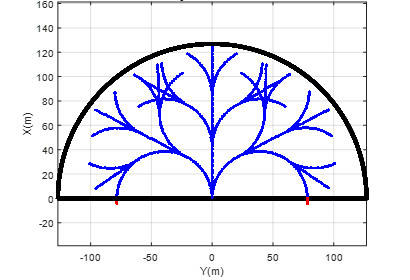
\includegraphics[width=\columnwidth]{Figs/PathPossibilities.png}
	\caption{\small Potential Paths predicted by 2-DOF Internal Vehicle Controller Model}  
	\label{fig:PossiblePaths}
\end{figure}

\todo[inline]{insert description of the point in polygon algorithm used for this study}
 
%% ------------------------------------------------------------

\subsection{Multi-DOF Vehicle Dynamics Models}\label{ss:IntModel}

The vehicle models embedded in the MPC are simplifications of the full, multi-body based, {\CHRONO} wheeled vehicle model which is being controlled.  Two models were considered initially, providing different levels of fidelity, as described below.

%% ------------------------------------------------------------

\subsubsection{2-DOF Vehicle Model}\label{sss:2DOFModel}
The standard vehicle model used in recently developed MPC obstacle avoidance algorithms such as~\cite{ModelFidelity2016} is the 2-DOF yaw plane vehicle model. These models normally either assume constant cornering stiffness or the nonlinear Pacejka Magic Formula Tire Model~\cite{Pacejka1997} to predict the ground tire interaction forces. For this study, the Pacejka Magic Formula is used to predict tire forces in the vehicle models.   

\todo[inline]{insert brief description of the Pacejka Magic Formula Tire Prediction Forces, maybe provide only the equations and leave the derivation to the sources}

A visual representation of the 2-DOF yaw plane vehicle model can be found in Fig.~\ref{fig:2DOF}. The 2-DOF model is described by the following first-order ordinary differential equations:

\begin{equation}\label{e:2DOF_Vdot}
\dot{V} = \left(F_{y,f} + F_{y,r}\right)/{M - U_0r} 
\end{equation}
\begin{equation}\label{e:2DOF_rdot}
\dot{r} = \left(F_{y,f} - F_{y,r}\right)/I_{zz}
\end{equation}
\begin{equation}\label{e:2DOF_psidot}
\dot{\psi} = r 
\end{equation}
\begin{equation}\label{e:2DOF_xdot}
\dot{x} = U_0\cos{\psi}-\left(V+L_fr\right)\sin{\psi}
\end{equation}
\begin{equation}\label{e:2DOF_ydot}
\dot{y} = U_0\sin{\psi}+\left(V+L_fr\right)\cos{\psi} \,,
\end{equation}
%
where $F_{y,f}$ and $F_{y,r}$ are the lateral tire forces at the front and rear axles, respectively. $U_0$ and $V$ are the longitudinal speed and lateral speed of the vehicle in the vehicle's coordinate frame. $\psi$ is the yaw angle and $r$ is the yaw rate. $\left(x,y\right)$ represent the front center location of the vehicle expressed in global coordinates. $M$ is vehicle mass, $I_{zz}$ is the moment of inertia of the vehicle, $L_f$ is the distance from the front axle to the vehicle CoG, and $L_r$ is the distance from the rear axle to the vehicle CoG. For this research, the model is constrained to a constant longitudinal speed. Then the planar 3-DOF body with one constraint results in the 2-DOF model used for this study.

\begin{figure}
	\centering
	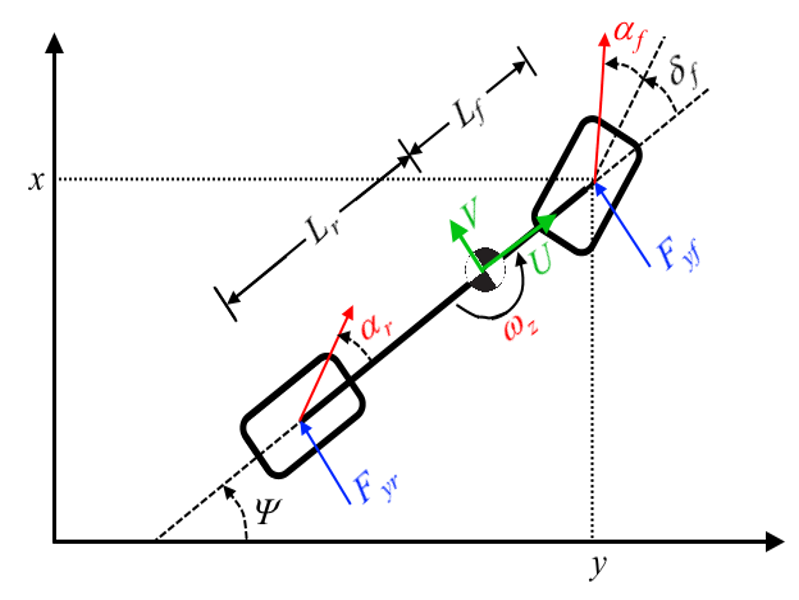
\includegraphics[width=1.0\columnwidth]{Figs/2DOF_haraus.png}
	\caption{\small 2-DOF Vehicle Model}  
	\label{fig:2DOF}
\end{figure}

%% ------------------------------------------------------------

\subsubsection{14-DOF Vehicle Model}\label{sss:14DOFModel}
A 14-DOF model is often used in studies such as these to test the obstacle avoidance controller with a higher fidelity vehicle model~\cite{ModelFidelity2016, ModelFidelity2013}. A benefit of using the 14-DOF in the controller is the model's ability to predict tire liftoff and account for dynamic effects from suspension systems. For this paper, it is appropriate to also compare performance of the local obstacle avoidance controller running an internal 14-DOF on rigid terrain versus granular terrain.  

The 14-DOF vehicle model consists of one sprung mass connected above four unsprung masses~\cite{RollStudies2007}. The sprung mass is allowed to roll, pitch, and yaw while also displacing laterally, vertically, and longitudinally. This sprung mass contributes six DOF to the model. Each of the four wheels are allowed to bounce vertically and rotate about the wheel horizontal axis. The front two wheels are also free to steer. Each wheel then contributes two DOF to the fourteen DOF model. The model is constrained at a constant longitudinal speed of 8.1 m/s. The equations used for this model, as well as their derivation can be found in~\cite{RollStudies2007}.

\todo[inline]{consider actually putting in the equations used for the 14DOF vehicle model here}

%%-------------------------------------------------------------

\subsection{Optimization Problem: Exhaustive Search Space}\label{ss:Optimization}

\todo[inline]{insert description of the exhaustive search space method used to find the optimal solution in this study}


%%============================================================

\section{Experimental Setup}\label{s:ExpSetup}

\subsection{Evaluation Metrics}\label{ss:Metrics}
Five evaluation metrics will be used to compare one test performance to the other. First, all test runs will be compared based on the time to reach the target, $T_{target}$ to determine which controller leads the vehicle to the target point quickest. Second, the closest distance the vehicle reaches to any obstacle, $d_{min}$, will be measured. Third, the control effort will be calculated and compared between test cases. The better test case will have a lower controller effort value. Finally, the maximum and average lateral accelerations will be calculated and compared. The accelerations are calculated at the driver's position in the chassis. Using the DEM-P method of simulation results in noisy acceleration data. To address this, acceleration data is filtered to remove noise. These five evaluation metrics provide a consistent methodology for comparing one test case with another, regardless of the terrain type and underlying analytical controller model.

The model to be controlled (the {\em plant}) is a full-vehicle {\ChronoVehicle} model of an HMMWV, which includes multi-body subsystems for the suspensions, steering, driveline, and powertrain, and is available in the {\CHRONO} package.

This vehicle model (see Fig.~\ref{fig:hmmwv}) has a curb weight of $2,550$~kg.
%
It includes independent front and rear double wishbone suspensions and a Pitman arm steering mechanism. The shock absorber and coil spring, mounted between the lower control arm and the chassis, are modeled with {\CHRONO} nonlinear force elements and include the effects of bump stops.
%
\begin{figure}
	\centering
	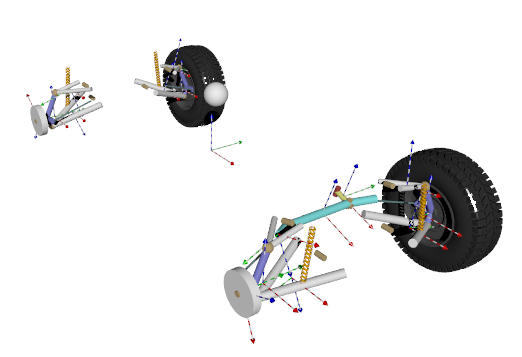
\includegraphics[width=\columnwidth]{Figs/hmmwv_bodies.png}
	\caption{\small Full-vehicle HMMWV multibody model.}  
	\label{fig:hmmwv}
\end{figure}

The AWD driveline is modeled using {\CHRONO} shaft elements and includes three power splitting elements (a central differential and front/rear differentials), as well as conical gears connected through 1-dimensional shaft elements which carry rotational inertia. 
%
The powertrain is also modeled using 1-dimensional shaft elements and includes models for a thermal engine specified through speed-torque maps for power and engine losses, a torque converter specified via maps for the capacity factor and the torque ratio, and an automatic transmission gearbox with three forward gears and a single reverse gear.
%
The connection between powertrain and driveline is a force-displacement interface at the driveshaft (with torque applied from the powertrain and angular velocity provided by the driveline).

For mobility studies on deformable terrain, provided that the tire inflation pressure is comparable or larger than the average ground pressure, according to the postulate by Wong~\cite{wong93} the tire can be considered in a so-called {\em rigid regime}.  As such, tire deformation can be ignored and the vehicle's tires modeled using rigid contact shapes.  The HMMWV tire model used here is thus represented by a cylinder with a radius of $0.47$~m ($18.5$~in) and a width of $0.254$~m ($10$~in).

%%-------------------------------------------------------------

\subsection{Simulation Parameters}\label{ss:SimParameters}

\begin{table}
\begin{center}
	\begin{tabular}{||c |c | c||} 
		\hline
		Test  & Terrain  & Controller Vehicle \\
		Number &  Type & Model\\ [0.5ex] 	
		\hline\hline
		1 & Rigid & 2-DOF \\ 
		\hline
		2 & Rigid & 14-DOF \\
		\hline
		3 & Granular & 2-DOF \\
		\hline
		4 & Granular & 14-DOF \\
		\hline
	\end{tabular}
\end{center}
\caption{Individual Simulation Test Information}
\label{t:TestMatrix}
\end{table}

Simulations on both rigid and granular terrain were compared to understand how the controller performs on non-ideal surfaces.  The two internal controller vehicle models studied in these tests were the previously described 2-DOF and 14-DOF vehicle models. All other controller parameters were kept unchanged over all tests. Referring to Table~\ref{t:TestMatrix}, the effect of model fidelity on controller performance was gauged by comparing test 1 with 2 and test 3 with 4, for rigid flat and granular terrain, respectively.
%%
Similarly, comparing test 1 with 3 and test 2 and 4 allowed evaluating the performance of each internal vehicle model on rigid and granular terrain.

\begin{figure}
	\centering
	\begin{subfigure}[b]{0.49\columnwidth}
		\centering
		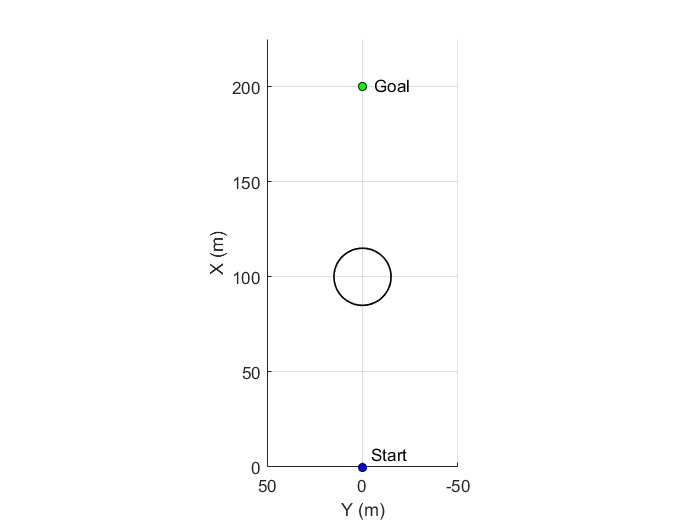
\includegraphics[width=\textwidth]{Figs/ObstacleField1.png}
		\caption{{\small Field 1}}   
		\label{fig:Obst1}
	\end{subfigure}
	\hfill
	\begin{subfigure}[b]{0.49\columnwidth}
		\centering
		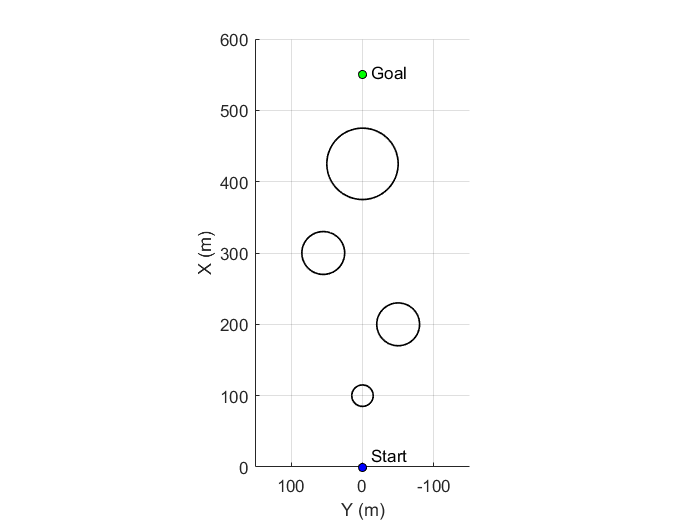
\includegraphics[width=\columnwidth]{Figs/ObstacleField2.png}
		\caption{\small Field 2}   
		\label{fig:Obst2}
	\end{subfigure}
	\caption{\small Obstacle fields.}
	\label{fig:Obst}
\end{figure}

Each of the above four tests consisted of runs on two fields with different obstacle distributions. 
%%
The first one, depicted in Fig.~\ref{fig:Obst1}, contains a single large circular obstacle located along the initial heading of the vehicle, with the target location at a large distance behind the obstacle. 
%%
The second obstacle field (see Fig.~\ref{fig:Obst2}) consists of four circular obstacles of varying sizes placed in the vehicle's initial heading direction, and provides a more realistic obstacle-avoidance scenario.
%%
Table~\ref{t:ObstSummary} summarizes the obstacle locations and dimensions, as well as the target location for the above two scenarios.

\begin{table}
	\begin{center}
		\begin{tabular}{||c|c|c|c||} 
			
			\hline
			& x & y & Radius\\
			& (m) & (m) & (m)\\
			\hline\hline
			\multicolumn{4}{||c||}{Field 1} \\
			\hline
			Target Location  & 200.0 & 0.0 & -\\ 
			\hline
			Obstacle 1 & 100.0 & 0.0 & 15.0\\			
			\hline\hline
			\multicolumn{4}{||c||}{Field 2} \\
			\hline
			Target Location  & 550.0 & 0.0 & -\\ 
			\hline
			Obstacle 1 & 100.0 & 0.0 & 15.0\\
			\hline
			Obstacle 2 & 200.0 & -50.0 & 30.0\\
			\hline
			Obstacle 3 & 300.0 & 55.0 & 30.0\\
			\hline
			Obstacle 4 & 425.0 & 0.0 & 50.0\\
			\hline
		\end{tabular}
	\end{center}
	\caption{Obstacle Field Parameters}
	\label{t:ObstSummary}
\end{table}

The following vehicle parameters are maintained throughout all of the executed tests. A PID speed controller is used to maintain a near constant speed of 8.1 m/s longitudinally for the simulated plant {\CHRONO} wheeled vehicle. This constant speed is also enforced in the analytical models internal to the MPC controller. The LIDAR sensor has a maximum range $R_{LIDAR} = 129.6~\text{m}$ and is sampled instantaneously at increments of $2.5^\circ$. The vehicle is limited to a maximum steering angle of $10^\circ$, with a maximum steering rate of $70^{\circ}/\text{s}$. 

%%-------------------------------------------------------------

\subsection{Rigid Terrain Simulation}\label{sss:RigidSim}

%%-------------------------------------------------------------

\subsection{Granular Terrain Simulation}\label{sss:GranSim}

Due to the large-scale nature of the simulations in this study, generating granular particles distributed across the entire obstacle field is both computationally exhausting and unreasonable. Instead, we adopt a moving-patch approach. Consider an AGV on a large terrain patch of $100$ by $100$ meters. Since we are primarily interested in the vehicle behavior and performance and not explicitly in the terrain behavior, we assume only a small patch of granular terrain underneath and around the vehicle is significant. This idea promoted the development of a relocating granular patch which enables simulations of a vehicle traversing granular terrain over a large area, without the need to generate particles everywhere throughout that area. 

\begin{figure}
	\centering
	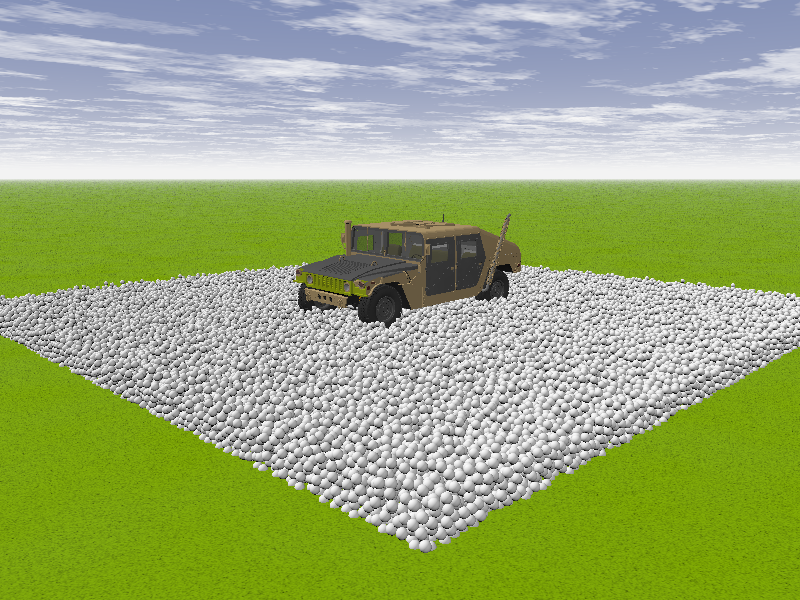
\includegraphics[width=0.8\columnwidth]{Figs/granPatch.png}
	\caption{\small Relocating Granular Patch that follows the vehicle}  
	\label{fig:granPatch}
\end{figure}

This mechanism allows a user to generate granular particles within a specified distance of the vehicle's CoG. Figure~\ref{fig:granPatch} presents the patch of granular terrain underneath the {\CHRONO}  HMMWV that moves with the vehicel. The particles are contained within four rigid walls to prevent them from escaping the desired terrain area. As the vehicle moves across the terrain, this patch maintains granular material underneath the vehicle by consistently relocating particles that are too far away from it. When the vehicle location comes within a certain predefined distance of any of the walls, a band of particles from the opposite end of the granular patch are relocated past the closest wall and all of the walls are shifted in that direction. Each of these relocation steps keeps the vehicle on top of granular terrain at all times. Depending on the vehicle, this granular patch can be resized for both computational efficiency and to guarantee the vehicle maintains a reasonable distance from the walls to prevent any boundary effects. This newly developed method of simulating granular terrain for AGV's is omnidirectional in the ground plane, allowing the vehicle to move in any direction while the terrain patch relocates and responds to that movement, thus enabling simulations over arbitrarily large areas.

For our simulations, the granular patch was maintained at a size of roughly $6.6$ by $6.6$ meters.  This number was assigned as two times the largest dimension of the vehicle.  The dimensions of the patch are not constant, however, since the patch expands in the direction of relocation by two times the largest particle radius every time the advancing wall is shifted.  This is done in order to avoid particle overlap, since the relocated particles are moved to a position that is shifted one largest particle radius ahead of the particles adjacent to the advancing wall.  After relocation, the walls of the granular patch are given a recovery velocity such that the granular patch regains its original dimensions in $0.1$ seconds.  This recovery time should be small relative to the duration of the simulations, and in general it will also depend on the velocity of the vehicle, since the granular patch should completely recover its dimensions between subsequent relocations.

Within the granular patch, the granular terrain was modeled by $55,931$ uniform spherical particles, with a micro-scale inter-particle sliding friction coefficient of $\mu = 0.8$, and particle diameter of $0.1$~m.  Previous studies~\cite{fleischmannetalGEGE2014} have shown that 
a randomly packed assembly of as few as $3,000$ - $30,000$ uniform spheres will exhibit macro-scale bulk granular material yield behavior (due to inter-particle sliding) that closely matches the Lade-Duncan yield surface, which is a well-established yield criterion in the field of geomechanics, where the macro-scale friction angle $\phi$ for the bulk granular material can be determined as a function of the inter-particle friction coefficient $\mu$.

Referring to Fig.~10 of~\cite{fleischmannetalGEGE2014}, a randomly packed assembly of uniform spheres with an inter-particle friction coefficient of $\mu = 0.8$ will exhibit macro-scale yield behavior corresponding to a bulk granular material with a macro-scale friction angle between roughly $35^\circ \leq \phi \leq 40^\circ$ if particle rotation is allowed (6 DOF particles), or with a macro-scale friction angle between roughly $65^\circ \leq \phi \leq 70^\circ$ if particle rotation is prohibited (3 DOF particles).
%
Since the granular patch used in our simulations contains more than $50,000$ uniform spheres, we can reliably conclude that it is accurately modeling the yield behavior of a true granular material on the macro-scale: either with a macro-scale friction angle of $35^\circ-40^\circ$ if particle rotation is allowed, which is typical of a wide range of dry natural and crushed sands \cite{Cho&Dodds&Santamarina2006}; or with a macro-scale friction angle of $65^\circ-70^\circ$ if particle rotation is prohibited, which is typical of crushed or fragmented rock, such as railway track ballast \cite{Indraratnaetal1998}.

We note that in the case of the HMMWV, the vehicle tire width is equal to only approximately $2.5$ particle diameters in the granular patch.  This is less than ideal.  However, a more suited value of $10$ particle diameters per tire width would increase the number of particles in the granular patch to more than $3$ million, which would result in prohibitively slow simulations, particularly for events corresponding to physical time durations on the order of $10$ seconds or more.



%% ============================================================

\section{EXPERIMENTAL RESULTS AND DISCUSSION}\label{s:results}

This section summarizes the results of the four tests listed in Table~\ref{t:TestMatrix}. 

\begin{figure}
	\centering
	\begin{subfigure}[b]{\columnwidth}
		\centering
		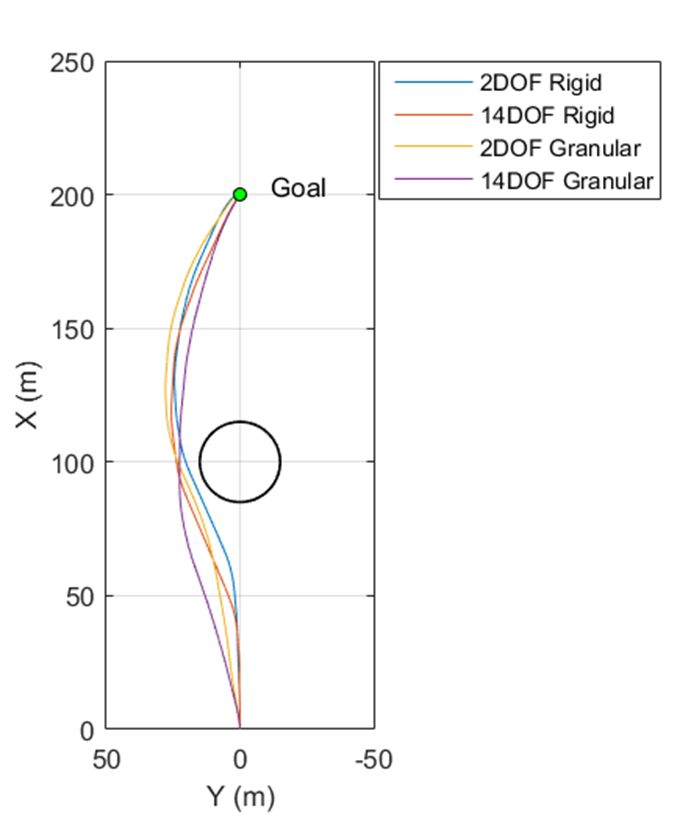
\includegraphics[height=\columnwidth]{Figs/ObstacleField1Trajectories.png}
		\caption{{\small Vehicle trajectories.}}   
		\label{fig:ObstacleField1Trajectories}
	\end{subfigure}
	\hfill
	\begin{subfigure}[b]{\columnwidth}
		\centering
		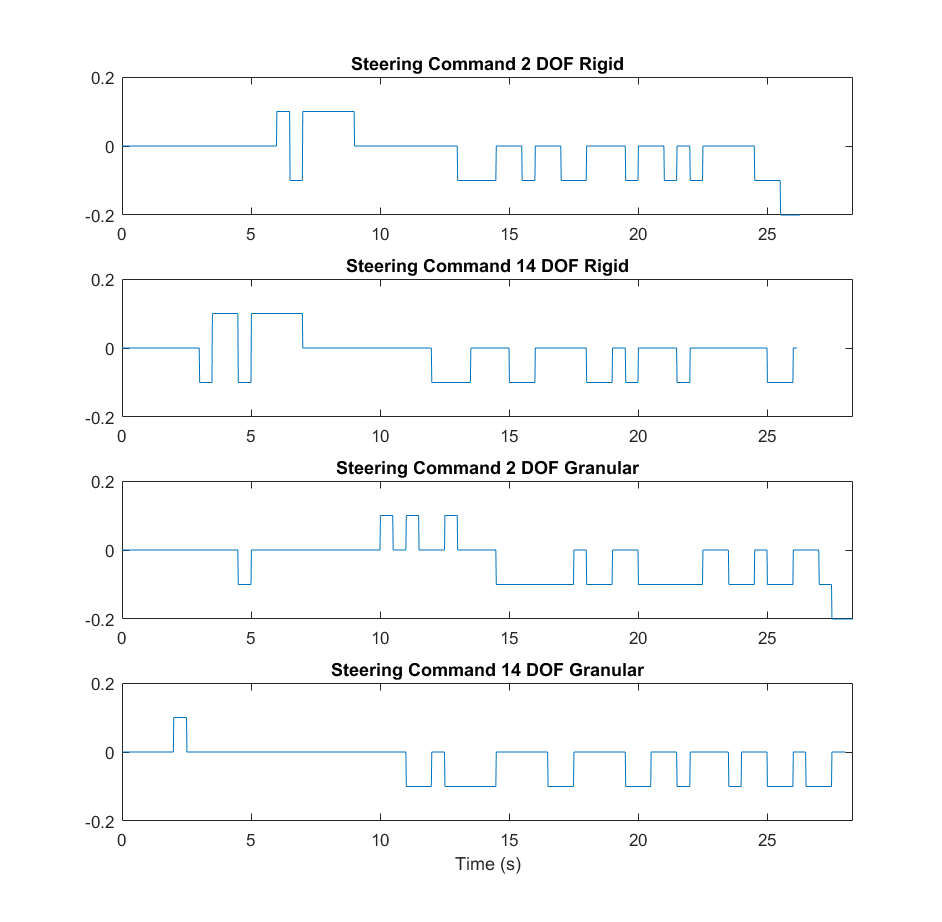
\includegraphics[width=\columnwidth]{Figs/SteeringCommandsField1.png}
		\caption{\small Steering commands.}   
		\label{fig:SteeringCommandsField1}
	\end{subfigure}
	\caption{\small Test results on obstacle field 1.}
	\label{fig:Obst1TestData}
\end{figure}

\begin{figure}
	\centering
	\begin{subfigure}[b]{\columnwidth}
		\centering
		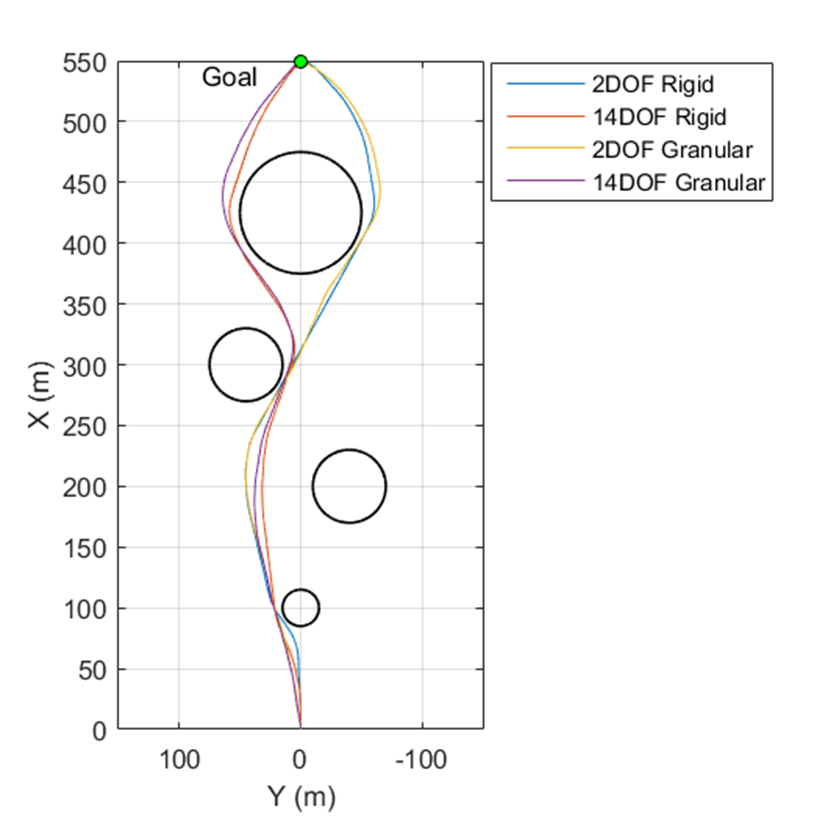
\includegraphics[height=\columnwidth]{Figs/ObstacleField2Trajectories.png}
		\caption{{\small Vehicle trajectories.}}   
		\label{fig:ObstacleField2Trajectories}
	\end{subfigure}
	\hfill
	\begin{subfigure}[b]{\columnwidth}
		\centering
		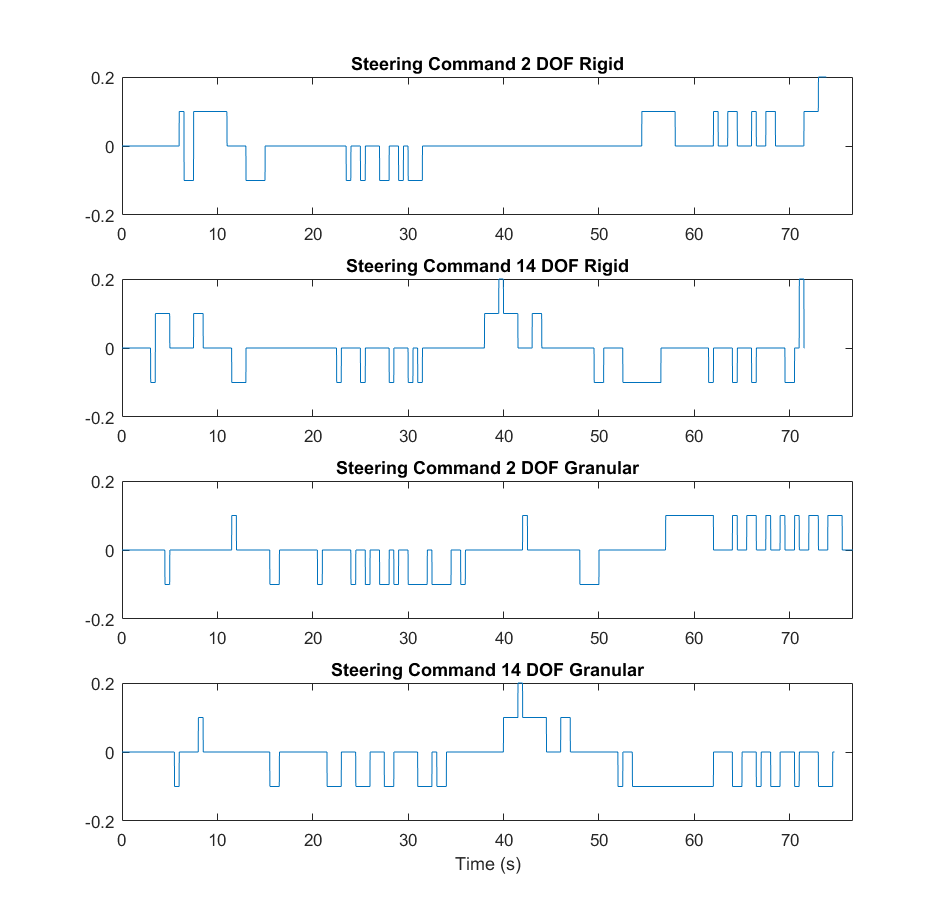
\includegraphics[width=\columnwidth]{Figs/SteeringCommandsField2.png}
		\caption{\small Steering commands.}   
		\label{fig:SteeringCommandsField2}
	\end{subfigure}
	\caption{\small Test results on obstacle field 2.}
	\label{fig:Obst2TestData}
\end{figure}

\begin{table*}
		\centering
\begin{tabular}{ ||p{6cm}|p{1.8cm}|p{1.8cm}|p{1.8cm}|p{1.8cm}||  }
		\hline
		Test Number & 1 & 2 & 3 & 4\\
		\hline
		Controller Model & 2-DOF & 14-DOF & 2-DOF & 14-DOF\\
		\hline
		Terrain & Rigid & Rigid & Granular & Granular\\
		\hline
		Time to Target (s)  & 26.67 & 26.15 & 28.32 & 28.03\\ 
		\hline
		Minimum Obstacle Distance (m) & 0.897 & 5.462 & 3.491 & 4.721\\
		\hline
		Controller Effort & 0.0340 & 0.0340 & 0.0340 & 0.0306\\
		\hline
		Max. Lateral Acceleration (m/s$^{2}$)& 2.78 & 1.57 & 2.47 & 2.33 \\
		\hline
		Avg. Lateral Acceleration (m/s$^{2}$) &0.54 & 0.51 & 0.55 & 0.46\\
		\hline
\end{tabular}
\caption{Test Evaluation Metrics Summary on Obstacle Field 1}
\label{t:EvalMetricsObst1}
\end{table*}

\begin{table*}
		\centering
\begin{tabular}{ ||p{6cm}|p{1.8cm}|p{1.8cm}|p{1.8cm}|p{1.8cm}||  }
		\hline
		Test Number & 1 & 2 & 3 & 4\\
		\hline
		Controller Model & 2-DOF & 14-DOF & 2-DOF & 14-DOF\\
		\hline
		Terrain & Rigid & Rigid & Granular & Granular\\
		\hline
		Time to Target (s)  & 73.85 & 71.55 & 76.64 & 74.70\\ 
		\hline
		Minimum Obstacle Distance (m) & 0.331 & 2.599 & 1.083 & 1.152\\
		\hline
		Controller Effort & 0.0510 & 0.0680 & 0.0714 & 0.0612\\
		\hline
		Max. Lateral Acceleration (m/s$^{2}$)& 2.92 & 2.51 & 2.55 & 2.45 \\
		\hline
		Avg. Lateral Acceleration (m/s$^{2}$) & 0.41 & 0.43 & 0.53 & 0.58\\
		\hline
\end{tabular}
\caption{Test Evaluation Metrics Summary on Obstacle Field 2.}
\label{t:EvalMetricsObst2}
\end{table*}

The trajectories for the four performed tests are presented in Figs.~\ref{fig:ObstacleField1Trajectories} and \ref{fig:ObstacleField2Trajectories}, for obstacle fields 1 and 2, respectively. The associated steering commands generated by the controller are presented in Figs.~\ref{fig:SteeringCommandsField1} and \ref{fig:SteeringCommandsField2}. 

The evaluation metrics for each test, as defined in Section~\ref{ss:Metrics}, are tabulated for each obstacle field in Tables~\ref{t:EvalMetricsObst1} and \ref{t:EvalMetricsObst2}. 

\subsection{Influence of model fidelity}

Assessing the effect of internal vehicle model fidelity on controller performance when the vehicle navigates on rigid terrain (comparison of tests 1 and 2), we make the following observations:
\begin{itemize}
\item the 14-DOF model leads to marginally faster travel to the target location;
\item the 2-DOF model leads to trajectories with lower obstacle clearance;
\item the two models result in the same controller effort on the first obstacle course; however, the higher-fidelity 14-DOF model requires 33\% more controller effort on the second obstacle course, a consequence of its decision of performing a course change to negotiate the last obstacle;
\item the two models result in approximately the same number of command changes on both obstacle courses;
\item the 14-DOF model results in lower maximum lateral accelerations.
\end{itemize}


Overall, while the higher-fidelity internal model leads to marginally better performance, the 2-DOF model is perfectly suitable for use in MPC-based local obstacle avoidance on rigid terrain at non-extreme speeds, as it can safely navigate the vehicle to its end goal. These results support the findings and conclusions in~\cite{ModelFidelity2016} even though a different AGV is considered here.

A similar comparison can be made for the case of obstacle avoidance on granular terrain (tests 3 and 4).  As on rigid terrain, the higher fidelity model leads to faster travel to the end goal, larger clearances to the obstacles, and lower maximum lateral accelerations.  However, on granular terrain, the controller effort required by using the 14-DOF model is always lower than that required by the 2-DOF model.  We again conclude that using a higher-fidelity internal controller model leads to overall marginally better performance.

The 2-DOF and 14-DOF internal vehicle models were derived using rigid ground assumptions, yet they are still capable of successfully and safely navigating the simulated vehicle through an obstacle field on granular terrain. The monitored metrics indicate a slight drop in controller performance when using the 2-DOF model. However, these gains are outweighed by the benefits, in terms of required computational effort, offered by implementing the lower-fidelity 2-DOF model. 

\subsection{Influence of terrain type}

Turning next to evaluating the 14-DOF internal controller model when navigating on rigid versus granular terrain (comparison of tests 2 and 4), we draw the following conclusions:
\begin{itemize}
\item on both obstacle courses, the target can be reached faster when navigating on rigid terrain;
\item the resulting trajectories are slightly closer to the obstacles when navigating on granular terrain;
\item the required controller effort is lower when navigating on granular terrain;
\item the maximum lateral accelerations are similar on both types of terrain.
\end{itemize}

A similar analysis can be performed on the 2-DOF model when used to control a vehicle on either rigid or granular terrain (comparison of tests 1 and 3). Unlike the 14-DOF model, the simpler 2-DOF model does a better job of approaching the obstacles more closely when controlling a vehicle on rigid rather than on granular terrain. Related to this, the controller effort on rigid terrain (test 1) is lower than that required on granular terrain (test 3). 
%come up with some explanations for this

The forces the vehicle experiences from driving on granular terrain can be much different than forces on simple rigid ground. Examining Figs.~\ref{fig:ObstacleField1Trajectories} and \ref{fig:ObstacleField2Trajectories}, the vehicle navigating on granular terrain does not turn as sharply for a given steering command as the vehicle does on rigid ground terrain. To understand the different behavior between a vehicle driving on rigid and granular terrain, a parametric study should be performed analyzing the vehicle driving on a variety of granular terrains with different granular parameters. 

Tests 3 and 4 were performed on granular terrain modeled as randomly packed uniform spheres with an inter-particle friction coefficient of $\mu = 0.8$, diameter of 0.1m, and a macro-scale friction angle roughly in the range $65^\circ \leq \phi \leq 70^\circ$, with particle rotation prohibited. This granular material resembles railway track ballast. These same tests were attempted on the the same randomly packed uniform spheres with particle rotation allowed resulting in a macro-scale friction angle between $35^\circ \leq \phi \leq 40^\circ$. This granular material resembles a dry sand. The results of this second set of tests on dry sand are not plotted or tabulated because the vehicle failed to move from the initial position. Instead, the vehicle spins its wheels in place at its initial location, making no progress forward as the wheels slowly dig themselves down into the granular terrain. However, this may be due to the too large diameter spheres used for this study for computational reasons. Generally the MPC LIDAR-based constant speed local obstacle avoidance controller used in this study is not appropriate for use on all granular terrains. There are situations where a combined speed and steering controller similar to that described in~\cite{SpeedSteer2015}, or even some new speed and steering controller which accounts for terrain parameters and mobility information to better predict vehicle movement, would be required. Neither of the models used in the present study, the rigid ground 2-DOF yaw plane model nor the rigid ground 14-DOF vehicle models, were appropriate for predicting vehicle behavior and performance on dry sand.

%% ============================================================

\section{FINAL EXPERIMENT WITH NEW VEHICLE MODEL ON GRANULAR MATERIAL}\label{s:finalResults}

%% ============================================================

\section{CONCLUSIONS}\label{s:conclusion}

In this study, using the multibody physics API {\CHRONO} a simulation has been developed of a HMMWV driving through a user specified obstacle field towards a defined target location. Within this simulation, a MPC LIDAR based local obstacle avoidance controller has been implemented to navigate the vehicle around obstacles as it encounters them. The controller itself uses a simplified analytical vehicle model to predict the actual controlled {\CHRONO} vehicle states within a finite prediction horizon in order to determine the optimal path and steering sequence forward from the current vehicle state. A method of simulating granular terrain for this large obstacle field was developed and implemented for this study. Two separate MPC Algorithms were developed, one that uses a 2-DOF vehicle model to predict {\CHRONO} vehicle states and a 14-DOF model to do the same. These two controllers were used to navigate a {\CHRONO} HMMWV through two obstacle courses on both rigid terrain and then on granular terrain. The results were compared to understand what if any improvements need to be made to the MPC LIDAR based local obstacle avoidance controller to successfully control a vehicle on granular terrain. 

As in \cite{ModelFidelity2016}, the controller with the 14-DOF internal vehicle model performs marginally better than the controller with the 2-DOF internal vehicle model in all situations. However, tests with the 2-DOF controller prove that this controller can still successfully navigate a vehicle through an obstacle field when the vehicle is moving at non-extreme speeds. Using the 2-DOF controller also allows for faster calculation of optimal steering sequences which is required for eventual realtime implementation. Both of the controllers navigated the vehicle worse on granular terrain than on rigid ground terrain, but this is expected since the internal vehicle controller models were derived using rigid ground assumptions. This study also highlights the complexities introoduced to vehicle modeling when the terrain is no longer rigid. Looking at the vehicle trajectories and lateral accelerations on granular terrain, there are clear differences in tire ground interactions when the terrain is now granular. The terrain granular parameters affect the turning characteristics of the vehicle, acceleration abilities, and overall vehicle dynamic performance which is not control predictive with the currently used 2-DOF and 14-DOF analytical vehicle models. 

The results of this study are promising. Since the 2-DOF controller is able to navigate the {\CHRONO} vehicle on this study's granular terrain, then there is some small set of granular terrain on which a 2-DOF model is sufficient for predicting vehicle performance well enough to guide the vehicle successfully and safely to a target point. However, these results also emphasize the need for future research and studies relating to vehicle simulation on granular terrain. This same sort of study should be performed parametrically on a comprehensive set of different granular terrains to understand the difference between vehicle performance on rigid ground and granular terrain. From there, a new intermediate analytical model should be research and developed that is not as complex as the 14-DOF model but does take into account granuler parameters such as the friction angle. 

\subsection{Future Work}\label{FutureWork}

%% ============================================================
\newpage
\section{BIBLIOGRAPHY}\label{s:bibliography}

\bibliographystyle{unsrt}
\bibliography{references}

%% ============================================================
\newpage
\section{APPENDICES}\label{s:appendices}

%% ============================================================


\end{document}



